\documentclass[12pt]{article}

%packages
%\usepackage{latexsym}
\usepackage{graphicx}
\usepackage{wrapfig}
\usepackage{color}
\usepackage{amsmath}
\usepackage{dsfont}
\usepackage{placeins}
\usepackage{amssymb}
\usepackage{skull}
\usepackage{enumerate}
\usepackage{soul}
\usepackage{alphalph}
\usepackage{hyperref}
\usepackage{enumerate}
\usepackage{listings}
%\usepackage{fancyhdr}

%\fancyhf{} % clear all header and footers
%\renewcommand{\headrulewidth}{0pt} % remove the header rule
%\fancyfoot[LE, LO]{\thepage}


%\usepackage{pstricks,pst-node,pst-tree}

%\usepackage{algpseudocode}
%\usepackage{amsthm}
%\usepackage{hyperref}
%\usepackage{mathrsfs}
%\usepackage{amsfonts}
%\usepackage{bbding}
%\usepackage{listings}
%\usepackage{appendix}
\usepackage[margin=1in]{geometry}
%\geometry{papersize={8.5in,11in},total={6.5in,9in}}
%\usepackage{cancel}
%\usepackage{algorithmic, algorithm}

\definecolor{dkgreen}{rgb}{0,0.6,0}
\definecolor{gray}{rgb}{0.5,0.5,0.5}
\definecolor{mauve}{rgb}{0.58,0,0.82}
\lstset{ %
  language=R,                     % the language of the code
  basicstyle=\footnotesize,       % the size of the fonts that are used for the code
  numbers=left,                   % where to put the line-numbers
  numberstyle=\tiny\color{gray},  % the style that is used for the line-numbers
  stepnumber=1,                   % the step between two line-numbers. If it's 1, each line
                                  % will be numbered
  numbersep=5pt,                  % how far the line-numbers are from the code
  backgroundcolor=\color{white},  % choose the background color. You must add \usepackage{color}
  showspaces=false,               % show spaces adding particular underscores
  showstringspaces=false,         % underline spaces within strings
  showtabs=false,                 % show tabs within strings adding particular underscores
  frame=single,                   % adds a frame around the code
  rulecolor=\color{black},        % if not set, the frame-color may be changed on line-breaks within not-black text (e.g. commens (green here))
  tabsize=2,                      % sets default tabsize to 2 spaces
  captionpos=b,                   % sets the caption-position to bottom
  breaklines=true,                % sets automatic line breaking
  breakatwhitespace=false,        % sets if automatic breaks should only happen at whitespace
  title=\lstname,                 % show the filename of files included with \lstinputlisting;
                                  % also try caption instead of title
  keywordstyle=\color{blue},      % keyword style
  commentstyle=\color{dkgreen},   % comment style
  stringstyle=\color{mauve},      % string literal style
  escapeinside={\%*}{*)},         % if you want to add a comment within your code
  morekeywords={*,...}            % if you want to add more keywords to the set
}

\newcommand{\qu}[1]{``#1''}
\newcommand{\spc}[1]{\\ \vspace{#1cm}}

\newcounter{probnum}
\setcounter{probnum}{1}
\newcounter{numpts}
\setcounter{numpts}{0}

%create definition to allow local margin changes
\def\changemargin#1#2{\list{}{\rightmargin#2\leftmargin#1}\item[]}
\let\endchangemargin=\endlist 

%allow equations to span multiple pages
\allowdisplaybreaks

%define colors and color typesetting conveniences
\definecolor{gray}{rgb}{0.5,0.5,0.5}
\definecolor{black}{rgb}{0,0,0}
\definecolor{white}{rgb}{1,1,1}
\definecolor{blue}{rgb}{0.5,0.5,1}
\newcommand{\inblue}[1]{\color{blue}#1 \color{black}}
\definecolor{green}{rgb}{0.133,0.545,0.133}
\newcommand{\ingreen}[1]{\color{green}#1 \color{black}}
\definecolor{yellow}{rgb}{1,0.549,0}
\newcommand{\inyellow}[1]{\color{yellow}#1 \color{black}}
\definecolor{red}{rgb}{1,0.133,0.133}
\newcommand{\inred}[1]{\color{red}#1 \color{black}}
\definecolor{purple}{rgb}{0.58,0,0.827}
\newcommand{\inpurple}[1]{\color{purple}#1 \color{black}}
\definecolor{gray}{rgb}{0.5,0.5,0.5}
\newcommand{\ingray}[1]{\color{gray}#1 \color{black}}
\definecolor{backgcode}{rgb}{0.97,0.97,0.8}
\definecolor{Brown}{cmyk}{0,0.81,1,0.60}
\definecolor{OliveGreen}{cmyk}{0.64,0,0.95,0.40}
\definecolor{CadetBlue}{cmyk}{0.62,0.57,0.23,0}

%define new math operators
\DeclareMathOperator*{\argmax}{arg\,max~}
\DeclareMathOperator*{\argmin}{arg\,min~}
\DeclareMathOperator*{\argsup}{arg\,sup~}
\DeclareMathOperator*{\arginf}{arg\,inf~}
\DeclareMathOperator*{\convolution}{\text{\Huge{$\ast$}}}
\newcommand{\infconv}[2]{\convolution^\infty_{#1 = 1} #2}
%true functions

%%%% GENERAL SHORTCUTS

\makeatletter
\newalphalph{\alphmult}[mult]{\@alph}{26}
\renewcommand{\labelenumi}{(\alphmult{\value{enumi}})}
\renewcommand{\theenumi}{\AlphAlph{\value{enumi}}}
\makeatother
%shortcuts for pure typesetting conveniences
\newcommand{\bv}[1]{\boldsymbol{#1}}

%shortcuts for compound constants
\newcommand{\BetaDistrConst}{\dfrac{\Gamma(\alpha + \beta)}{\Gamma(\alpha)\Gamma(\beta)}}
\newcommand{\NormDistrConst}{\dfrac{1}{\sqrt{2\pi\sigma^2}}}

%shortcuts for conventional symbols
\newcommand{\tsq}{\tau^2}
\newcommand{\tsqh}{\hat{\tau}^2}
\newcommand{\sigsq}{\sigma^2}
\newcommand{\sigsqsq}{\parens{\sigma^2}^2}
\newcommand{\sigsqovern}{\dfrac{\sigsq}{n}}
\newcommand{\tausq}{\tau^2}
\newcommand{\tausqalpha}{\tau^2_\alpha}
\newcommand{\tausqbeta}{\tau^2_\beta}
\newcommand{\tausqsigma}{\tau^2_\sigma}
\newcommand{\betasq}{\beta^2}
\newcommand{\sigsqvec}{\bv{\sigma}^2}
\newcommand{\sigsqhat}{\hat{\sigma}^2}
\newcommand{\sigsqhatmlebayes}{\sigsqhat_{\text{Bayes, MLE}}}
\newcommand{\sigsqhatmle}[1]{\sigsqhat_{#1, \text{MLE}}}
\newcommand{\bSigma}{\bv{\Sigma}}
\newcommand{\bSigmainv}{\bSigma^{-1}}
\newcommand{\thetavec}{\bv{\theta}}
\newcommand{\thetahat}{\hat{\theta}}
\newcommand{\thetahatmle}{\hat{\theta}_{\mathrm{MLE}}}
\newcommand{\thetavechatmle}{\hat{\thetavec}_{\mathrm{MLE}}}
\newcommand{\muhat}{\hat{\mu}}
\newcommand{\musq}{\mu^2}
\newcommand{\muvec}{\bv{\mu}}
\newcommand{\muhatmle}{\muhat_{\text{MLE}}}
\newcommand{\lambdahat}{\hat{\lambda}}
\newcommand{\lambdahatmle}{\lambdahat_{\text{MLE}}}
\newcommand{\thetahatmap}{\hat{\theta}_{\mathrm{MAP}}}
\newcommand{\thetahatmae}{\hat{\theta}_{\mathrm{MAE}}}
\newcommand{\thetahatmmse}{\hat{\theta}_{\mathrm{MMSE}}}
\newcommand{\etavec}{\bv{\eta}}
\newcommand{\alphavec}{\bv{\alpha}}
\newcommand{\minimaxdec}{\delta^*_{\mathrm{mm}}}
\newcommand{\ybar}{\bar{y}}
\newcommand{\xbar}{\bar{x}}
\newcommand{\Xbar}{\bar{X}}
\newcommand{\iid}{~{\buildrel iid \over \sim}~}
\newcommand{\inddist}{~{\buildrel ind \over \sim}~}
\newcommand{\approxdist}{~{\buildrel approx \over \sim}~}
\newcommand{\equalsindist}{~{\buildrel d \over =}~}
\newcommand{\loglik}[1]{\ell\parens{#1}}
\newcommand{\thetahatkminone}{\thetahat^{(k-1)}}
\newcommand{\thetahatkplusone}{\thetahat^{(k+1)}}
\newcommand{\thetahatk}{\thetahat^{(k)}}
\newcommand{\half}{\frac{1}{2}}
\newcommand{\third}{\frac{1}{3}}
\newcommand{\twothirds}{\frac{2}{3}}
\newcommand{\fourth}{\frac{1}{4}}
\newcommand{\fifth}{\frac{1}{5}}
\newcommand{\sixth}{\frac{1}{6}}

%shortcuts for vector and matrix notation
\newcommand{\A}{\bv{A}}
\newcommand{\At}{\A^T}
\newcommand{\Ainv}{\inverse{\A}}
\newcommand{\B}{\bv{B}}
\newcommand{\K}{\bv{K}}
\newcommand{\Kt}{\K^T}
\newcommand{\Kinv}{\inverse{K}}
\newcommand{\Kinvt}{(\Kinv)^T}
\newcommand{\M}{\bv{M}}
\newcommand{\Bt}{\B^T}
\newcommand{\Q}{\bv{Q}}
\newcommand{\Qt}{\Q^T}
\newcommand{\R}{\bv{R}}
\newcommand{\Rt}{\R^T}
\newcommand{\Z}{\bv{Z}}
\newcommand{\X}{\bv{X}}
\newcommand{\Xsub}{\X_{\text{(sub)}}}
\newcommand{\Xsubadj}{\X_{\text{(sub,adj)}}}
\newcommand{\I}{\bv{I}}
\newcommand{\Y}{\bv{Y}}
\newcommand{\sigsqI}{\sigsq\I}
\renewcommand{\P}{\bv{P}}
\newcommand{\Psub}{\P_{\text{(sub)}}}
\newcommand{\Pt}{\P^T}
\newcommand{\Pii}{P_{ii}}
\newcommand{\Pij}{P_{ij}}
\newcommand{\IminP}{(\I-\P)}
\newcommand{\Xt}{\bv{X}^T}
\newcommand{\XtX}{\Xt\X}
\newcommand{\XtXinv}{\parens{\Xt\X}^{-1}}
\newcommand{\XtXinvXt}{\XtXinv\Xt}
\newcommand{\XXtXinvXt}{\X\XtXinvXt}
\newcommand{\x}{\bv{x}}
\newcommand{\w}{\bv{w}}
\newcommand{\onevec}{\bv{1}}
\newcommand{\oneton}{1, \ldots, n}
\newcommand{\yoneton}{y_1, \ldots, y_n}
\newcommand{\yonetonorder}{y_{(1)}, \ldots, y_{(n)}}
\newcommand{\Yoneton}{Y_1, \ldots, Y_n}
\newcommand{\iinoneton}{i \in \braces{\oneton}}
\newcommand{\onetom}{1, \ldots, m}
\newcommand{\jinonetom}{j \in \braces{\onetom}}
\newcommand{\xoneton}{x_1, \ldots, x_n}
\newcommand{\Xoneton}{X_1, \ldots, X_n}
\newcommand{\xt}{\x^T}
\newcommand{\y}{\bv{y}}
\newcommand{\yt}{\y^T}
\renewcommand{\c}{\bv{c}}
\newcommand{\ct}{\c^T}
\newcommand{\tstar}{\bv{t}^*}
\renewcommand{\u}{\bv{u}}
\renewcommand{\v}{\bv{v}}
\renewcommand{\a}{\bv{a}}
\newcommand{\s}{\bv{s}}
\newcommand{\yadj}{\y_{\text{(adj)}}}
\newcommand{\xjadj}{\x_{j\text{(adj)}}}
\newcommand{\xjadjM}{\x_{j \perp M}}
\newcommand{\yhat}{\hat{\y}}
\newcommand{\yhatsub}{\yhat_{\text{(sub)}}}
\newcommand{\yhatstar}{\yhat^*}
\newcommand{\yhatstarnew}{\yhatstar_{\text{new}}}
\newcommand{\z}{\bv{z}}
\newcommand{\zt}{\z^T}
\newcommand{\bb}{\bv{b}}
\newcommand{\bbt}{\bb^T}
\newcommand{\bbeta}{\bv{\beta}}
\newcommand{\beps}{\bv{\epsilon}}
\newcommand{\bepst}{\beps^T}
\newcommand{\e}{\bv{e}}
\newcommand{\Mofy}{\M(\y)}
\newcommand{\KofAlpha}{K(\alpha)}
\newcommand{\ellset}{\mathcal{L}}
\newcommand{\oneminalph}{1-\alpha}
\newcommand{\SSE}{\text{SSE}}
\newcommand{\SSEsub}{\text{SSE}_{\text{(sub)}}}
\newcommand{\MSE}{\text{MSE}}
\newcommand{\RMSE}{\text{RMSE}}
\newcommand{\SSR}{\text{SSR}}
\newcommand{\SST}{\text{SST}}
\newcommand{\JSest}{\delta_{\text{JS}}(\x)}
\newcommand{\Bayesest}{\delta_{\text{Bayes}}(\x)}
\newcommand{\EmpBayesest}{\delta_{\text{EmpBayes}}(\x)}
\newcommand{\BLUPest}{\delta_{\text{BLUP}}}
\newcommand{\MLEest}[1]{\hat{#1}_{\text{MLE}}}

%shortcuts for Linear Algebra stuff (i.e. vectors and matrices)
\newcommand{\twovec}[2]{\bracks{\begin{array}{c} #1 \\ #2 \end{array}}}
\newcommand{\threevec}[3]{\bracks{\begin{array}{c} #1 \\ #2 \\ #3 \end{array}}}
\newcommand{\fivevec}[5]{\bracks{\begin{array}{c} #1 \\ #2 \\ #3 \\ #4 \\ #5 \end{array}}}
\newcommand{\twobytwomat}[4]{\bracks{\begin{array}{cc} #1 & #2 \\ #3 & #4 \end{array}}}
\newcommand{\threebytwomat}[6]{\bracks{\begin{array}{cc} #1 & #2 \\ #3 & #4 \\ #5 & #6 \end{array}}}

%shortcuts for conventional compound symbols
\newcommand{\thetainthetas}{\theta \in \Theta}
\newcommand{\reals}{\mathbb{R}}
\newcommand{\complexes}{\mathbb{C}}
\newcommand{\rationals}{\mathbb{Q}}
\newcommand{\integers}{\mathbb{Z}}
\newcommand{\naturals}{\mathbb{N}}
\newcommand{\forallninN}{~~\forall n \in \naturals}
\newcommand{\forallxinN}[1]{~~\forall #1 \in \reals}
\newcommand{\matrixdims}[2]{\in \reals^{\,#1 \times #2}}
\newcommand{\inRn}[1]{\in \reals^{\,#1}}
\newcommand{\mathimplies}{\quad\Rightarrow\quad}
\newcommand{\mathlogicequiv}{\quad\Leftrightarrow\quad}
\newcommand{\eqncomment}[1]{\quad \text{(#1)}}
\newcommand{\limitn}{\lim_{n \rightarrow \infty}}
\newcommand{\limitN}{\lim_{N \rightarrow \infty}}
\newcommand{\limitd}{\lim_{d \rightarrow \infty}}
\newcommand{\limitt}{\lim_{t \rightarrow \infty}}
\newcommand{\limitsupn}{\limsup_{n \rightarrow \infty}~}
\newcommand{\limitinfn}{\liminf_{n \rightarrow \infty}~}
\newcommand{\limitk}{\lim_{k \rightarrow \infty}}
\newcommand{\limsupn}{\limsup_{n \rightarrow \infty}}
\newcommand{\limsupk}{\limsup_{k \rightarrow \infty}}
\newcommand{\floor}[1]{\left\lfloor #1 \right\rfloor}
\newcommand{\ceil}[1]{\left\lceil #1 \right\rceil}

%shortcuts for environments
\newcommand{\beqn}{\vspace{-0.25cm}\begin{eqnarray*}}
\newcommand{\eeqn}{\end{eqnarray*}}
\newcommand{\bneqn}{\vspace{-0.25cm}\begin{eqnarray}}
\newcommand{\eneqn}{\end{eqnarray}}
\newcommand{\benum}{\begin{enumerate}}
\newcommand{\eenum}{\end{enumerate}}

%shortcuts for mini environments
\newcommand{\parens}[1]{\left(#1\right)}
\newcommand{\squared}[1]{\parens{#1}^2}
\newcommand{\tothepow}[2]{\parens{#1}^{#2}}
\newcommand{\prob}[1]{\mathbb{P}\parens{#1}}
\newcommand{\littleo}[1]{o\parens{#1}}
\newcommand{\bigo}[1]{O\parens{#1}}
\newcommand{\Lp}[1]{\mathbb{L}^{#1}}
\renewcommand{\arcsin}[1]{\text{arcsin}\parens{#1}}
\newcommand{\prodonen}[2]{\bracks{\prod_{#1=1}^n #2}}
\newcommand{\mysum}[4]{\sum_{#1=#2}^{#3} #4}
\newcommand{\sumonen}[2]{\sum_{#1=1}^n #2}
\newcommand{\infsum}[2]{\sum_{#1=1}^\infty #2}
\newcommand{\infprod}[2]{\prod_{#1=1}^\infty #2}
\newcommand{\infunion}[2]{\bigcup_{#1=1}^\infty #2}
\newcommand{\infinter}[2]{\bigcap_{#1=1}^\infty #2}
\newcommand{\infintegral}[2]{\int^\infty_{-\infty} #2 ~\text{d}#1}
\newcommand{\supthetas}[1]{\sup_{\thetainthetas}\braces{#1}}
\newcommand{\bracks}[1]{\left[#1\right]}
\newcommand{\braces}[1]{\left\{#1\right\}}
\newcommand{\set}[1]{\left\{#1\right\}}
\newcommand{\abss}[1]{\left|#1\right|}
\newcommand{\norm}[1]{\left|\left|#1\right|\right|}
\newcommand{\normsq}[1]{\norm{#1}^2}
\newcommand{\inverse}[1]{\parens{#1}^{-1}}
\newcommand{\rowof}[2]{\parens{#1}_{#2\cdot}}

%shortcuts for functionals
\newcommand{\realcomp}[1]{\text{Re}\bracks{#1}}
\newcommand{\imagcomp}[1]{\text{Im}\bracks{#1}}
\newcommand{\range}[1]{\text{range}\bracks{#1}}
\newcommand{\colsp}[1]{\text{colsp}\bracks{#1}}
\newcommand{\rowsp}[1]{\text{rowsp}\bracks{#1}}
\newcommand{\tr}[1]{\text{tr}\bracks{#1}}
\newcommand{\rank}[1]{\text{rank}\bracks{#1}}
\newcommand{\proj}[2]{\text{Proj}_{#1}\bracks{#2}}
\newcommand{\projcolspX}[1]{\text{Proj}_{\colsp{\X}}\bracks{#1}}
\newcommand{\median}[1]{\text{median}\bracks{#1}}
\newcommand{\mean}[1]{\text{mean}\bracks{#1}}
\newcommand{\dime}[1]{\text{dim}\bracks{#1}}
\renewcommand{\det}[1]{\text{det}\bracks{#1}}
\newcommand{\expe}[1]{\mathbb{E}\bracks{#1}}
\newcommand{\expeabs}[1]{\expe{\abss{#1}}}
\newcommand{\expesub}[2]{\mathbb{E}_{#1}\bracks{#2}}
\newcommand{\cexpesub}[3]{\mathbb{E}_{#1}\bracks{#2~|~#3}}
\newcommand{\indic}[1]{\mathds{1}_{#1}}
\newcommand{\var}[1]{\mathbb{V}\text{ar}\bracks{#1}}
\newcommand{\sd}[1]{\mathbb{S}\text{D}\bracks{#1}}
\newcommand{\cov}[2]{\text{Cov}\bracks{#1, #2}}
\newcommand{\corr}[2]{\text{Corr}\bracks{#1, #2}}
\newcommand{\se}[1]{\text{SE}\bracks{#1}}
\newcommand{\seest}[1]{\hat{\text{SE}}\bracks{#1}}
\newcommand{\bias}[1]{\text{Bias}\bracks{#1}}
\newcommand{\partialop}[2]{\dfrac{\partial}{\partial #1}\bracks{#2}}
\newcommand{\secpartialop}[2]{\dfrac{\partial^2}{\partial #1^2}\bracks{#2}}
\newcommand{\mixpartialop}[3]{\dfrac{\partial^2}{\partial #1 \partial #2}\bracks{#3}}

%shortcuts for functions
\renewcommand{\exp}[1]{\mathrm{exp}\parens{#1}}
\renewcommand{\cos}[1]{\text{cos}\parens{#1}}
\renewcommand{\sin}[1]{\text{sin}\parens{#1}}
\newcommand{\sign}[1]{\text{sign}\parens{#1}}
\newcommand{\are}[1]{\mathrm{ARE}\parens{#1}}
\newcommand{\natlog}[1]{\ln\parens{#1}}
\newcommand{\oneover}[1]{\frac{1}{#1}}
\newcommand{\overtwo}[1]{\frac{#1}{2}}
\newcommand{\overn}[1]{\frac{#1}{n}}
\newcommand{\oneoversqrt}[1]{\oneover{\sqrt{#1}}}
\newcommand{\sqd}[1]{\parens{#1}^2}
\newcommand{\loss}[1]{\ell\parens{\theta, #1}}
\newcommand{\losstwo}[2]{\ell\parens{#1, #2}}
\newcommand{\cf}{\phi(t)}

%English language specific shortcuts
\newcommand{\ie}{\textit{i.e.} }
\newcommand{\AKA}{\textit{AKA} }
\renewcommand{\iff}{\textit{iff}}
\newcommand{\eg}{\textit{e.g.} }
\renewcommand{\st}{\textit{s.t.} }
\newcommand{\wrt}{\textit{w.r.t.} }
\newcommand{\mathst}{~~\text{\st}~~}
\newcommand{\mathand}{~~\text{and}~~}
\newcommand{\ala}{\textit{a la} }
\newcommand{\ppp}{posterior predictive p-value}
\newcommand{\dd}{dataset-to-dataset}

%shortcuts for distribution titles
\newcommand{\logistic}[2]{\mathrm{Logistic}\parens{#1,\,#2}}
\newcommand{\bernoulli}[1]{\mathrm{Bernoulli}\parens{#1}}
\newcommand{\betanot}[2]{\mathrm{Beta}\parens{#1,\,#2}}
\newcommand{\stdbetanot}{\betanot{\alpha}{\beta}}
\newcommand{\multnormnot}[3]{\mathcal{N}_{#1}\parens{#2,\,#3}}
\newcommand{\normnot}[2]{\mathcal{N}\parens{#1,\,#2}}
\newcommand{\classicnormnot}{\normnot{\mu}{\sigsq}}
\newcommand{\stdnormnot}{\normnot{0}{1}}
\newcommand{\uniform}[2]{\mathrm{U}\parens{#1,\,#2}}
\newcommand{\stduniform}{\uniform{0}{1}}
\newcommand{\exponential}[1]{\mathrm{Exp}\parens{#1}}
\newcommand{\gammadist}[2]{\mathrm{Gamma}\parens{#1, #2}}
\newcommand{\poisson}[1]{\mathrm{Poisson}\parens{#1}}
\newcommand{\binomial}[2]{\mathrm{Binomial}\parens{#1,\,#2}}
\newcommand{\rayleigh}[1]{\mathrm{Rayleigh}\parens{#1}}
\newcommand{\multinomial}[2]{\mathrm{Multinomial}\parens{#1,\,#2}}
\newcommand{\gammanot}[2]{\mathrm{Gamma}\parens{#1,\,#2}}
\newcommand{\cauchynot}[2]{\text{Cauchy}\parens{#1,\,#2}}
\newcommand{\invchisqnot}[1]{\text{Inv}\chisq{#1}}
\newcommand{\invscaledchisqnot}[2]{\text{ScaledInv}\ncchisq{#1}{#2}}
\newcommand{\invgammanot}[2]{\text{InvGamma}\parens{#1,\,#2}}
\newcommand{\chisq}[1]{\chi^2_{#1}}
\newcommand{\ncchisq}[2]{\chi^2_{#1}\parens{#2}}
\newcommand{\ncF}[3]{F_{#1,#2}\parens{#3}}

%shortcuts for PDF's of common distributions
\newcommand{\logisticpdf}[3]{\oneover{#3}\dfrac{\exp{-\dfrac{#1 - #2}{#3}}}{\parens{1+\exp{-\dfrac{#1 - #2}{#3}}}^2}}
\newcommand{\betapdf}[3]{\dfrac{\Gamma(#2 + #3)}{\Gamma(#2)\Gamma(#3)}#1^{#2-1} (1-#1)^{#3-1}}
\newcommand{\normpdf}[3]{\frac{1}{\sqrt{2\pi#3}}\exp{-\frac{1}{2#3}(#1 - #2)^2}}
\newcommand{\normpdfvarone}[2]{\dfrac{1}{\sqrt{2\pi}}e^{-\half(#1 - #2)^2}}
\newcommand{\chisqpdf}[2]{\dfrac{1}{2^{#2/2}\Gamma(#2/2)}\; {#1}^{#2/2-1} e^{-#1/2}}
\newcommand{\invchisqpdf}[2]{\dfrac{2^{-\overtwo{#1}}}{\Gamma(#2/2)}\,{#1}^{-\overtwo{#2}-1}  e^{-\oneover{2 #1}}}
\newcommand{\uniformdiscrete}[1]{\mathrm{Uniform}\parens{\braces{#1}}}
\newcommand{\exponentialpdf}[2]{#2\exp{-#2#1}}
\newcommand{\poissonpdf}[2]{\dfrac{e^{-#1} #1^{#2}}{#2!}}
\newcommand{\binomialpdf}[3]{\binom{#2}{#1}#3^{#1}(1-#3)^{#2-#1}}
\newcommand{\rayleighpdf}[2]{\dfrac{#1}{#2^2}\exp{-\dfrac{#1^2}{2 #2^2}}}
\newcommand{\gammapdf}[3]{\dfrac{#3^#2}{\Gamma\parens{#2}}#1^{#2-1}\exp{-#3 #1}}
\newcommand{\cauchypdf}[3]{\oneover{\pi} \dfrac{#3}{\parens{#1-#2}^2 + #3^2}}
\newcommand{\Gammaf}[1]{\Gamma\parens{#1}}

%shortcuts for miscellaneous typesetting conveniences
\newcommand{\notesref}[1]{\marginpar{\color{gray}\tt #1\color{black}}}

%%%% DOMAIN-SPECIFIC SHORTCUTS

%Real analysis related shortcuts
\newcommand{\zeroonecl}{\bracks{0,1}}
\newcommand{\forallepsgrzero}{\forall \epsilon > 0~~}
\newcommand{\lessthaneps}{< \epsilon}
\newcommand{\fraccomp}[1]{\text{frac}\bracks{#1}}

%Bayesian related shortcuts
\newcommand{\yrep}{y^{\text{rep}}}
\newcommand{\yrepisq}{(\yrep_i)^2}
\newcommand{\yrepvec}{\bv{y}^{\text{rep}}}


%Probability shortcuts
\newcommand{\SigField}{\mathcal{F}}
\newcommand{\ProbMap}{\mathcal{P}}
\newcommand{\probtrinity}{\parens{\Omega, \SigField, \ProbMap}}
\newcommand{\convp}{~{\buildrel p \over \rightarrow}~}
\newcommand{\convLp}[1]{~{\buildrel \Lp{#1} \over \rightarrow}~}
\newcommand{\nconvp}{~{\buildrel p \over \nrightarrow}~}
\newcommand{\convae}{~{\buildrel a.e. \over \longrightarrow}~}
\newcommand{\convau}{~{\buildrel a.u. \over \longrightarrow}~}
\newcommand{\nconvau}{~{\buildrel a.u. \over \nrightarrow}~}
\newcommand{\nconvae}{~{\buildrel a.e. \over \nrightarrow}~}
\newcommand{\convd}{~{\buildrel \mathcal{D} \over \rightarrow}~}
\newcommand{\nconvd}{~{\buildrel \mathcal{D} \over \nrightarrow}~}
\newcommand{\withprob}{~~\text{w.p.}~~}
\newcommand{\io}{~~\text{i.o.}}

\newcommand{\Acl}{\bar{A}}
\newcommand{\ENcl}{\bar{E}_N}
\newcommand{\diam}[1]{\text{diam}\parens{#1}}

\newcommand{\taua}{\tau_a}

\newcommand{\myint}[4]{\int_{#2}^{#3} #4 \,\text{d}#1}
\newcommand{\laplacet}[1]{\mathscr{L}\bracks{#1}}
\newcommand{\laplaceinvt}[1]{\mathscr{L}^{-1}\bracks{#1}}
\renewcommand{\min}[1]{\text{min}\braces{#1}}

\newcommand{\Vbar}[1]{\bar{V}\parens{#1}}
\newcommand{\expnegrtau}{\exp{-r\tau}}
\newcommand{\cprob}[2]{\prob{#1~|~#2}}

%%% problem typesetting
\newcommand{\problem}{\vspace{0.2cm} \noindent {\large{\textsf{Problem \arabic{probnum}~}}} \addtocounter{probnum}{1}}
%\newcommand{\easyproblem}{\ingreen{\noindent \textsf{Problem \arabic{probnum}~}} \addtocounter{probnum}{1}}
%\newcommand{\intermediateproblem}{\noindent \inyellow{\textsf{Problem \arabic{probnum}~}} \addtocounter{probnum}{1}}
%\newcommand{\hardproblem}{\inred{\noindent \textsf{Problem \arabic{probnum}~}} \addtocounter{probnum}{1}}
%\newcommand{\extracreditproblem}{\noindent \inpurple{\textsf{Problem \arabic{probnum}~}} \addtocounter{probnum}{1}}

\newcommand{\easysubproblem}{\ingreen{\item}}
\newcommand{\intermediatesubproblem}{\inyellow{\item}}
\newcommand{\hardsubproblem}{\inred{\item}}
\newcommand{\extracreditsubproblem}{\inpurple{\item}}
%\newcommand{\subquestionwithpoints}[1]{\addtocounter{numpts}{#1} \item \ingray{[#1 pt]}~~} %  / \arabic{numpts} pts
\newcommand{\subquestionwithpoints}[1]{\addtocounter{numpts}{#1} \item \ingray{[#1 pt / \arabic{numpts} pts]}~~}  

\title{Math 390.4 / 650.3 Spring 2019 \\ Midterm Examination Two}
\author{Professor Adam Kapelner}

\date{Thursday, April 18, 2019}

\begin{document}
\maketitle

\noindent Full Name \line(1,0){410}

\thispagestyle{empty}

\section*{Code of Academic Integrity}

\footnotesize
Since the college is an academic community, its fundamental purpose is the pursuit of knowledge. Essential to the success of this educational mission is a commitment to the principles of academic integrity. Every member of the college community is responsible for upholding the highest standards of honesty at all times. Students, as members of the community, are also responsible for adhering to the principles and spirit of the following Code of Academic Integrity.

Activities that have the effect or intention of interfering with education, pursuit of knowledge, or fair evaluation of a student's performance are prohibited. Examples of such activities include but are not limited to the following definitions:

\paragraph{Cheating} Using or attempting to use unauthorized assistance, material, or study aids in examinations or other academic work or preventing, or attempting to prevent, another from using authorized assistance, material, or study aids. Example: using an unauthorized cheat sheet in a quiz or exam, altering a graded exam and resubmitting it for a better grade, etc.
\\

\noindent I acknowledge and agree to uphold this Code of Academic Integrity. \\

\begin{center}
\line(1,0){250} ~~~ \line(1,0){100}\\
~~~~~~~~~~~~~~~~~~~~~signature~~~~~~~~~~~~~~~~~~~~~~~~~~~~~~~~~~~~~~~~~~~~~ date
\end{center}

\normalsize

\section*{Instructions}

This exam is 110 minutes and closed-book. You are allowed \textbf{one} page (front and back) of a \qu{cheat sheet.} You may use a graphing calculator of your choice. Please read the questions carefully. If the question reads \qu{compute,} this means the solution will be a number otherwise you can leave the answer in \textit{any} widely accepted mathematical notation which could be resolved to an exact or approximate number with the use of a computer. I advise you to skip problems marked \qu{[Extra Credit]} until you have finished the other questions on the exam, then loop back and plug in all the holes. I also advise you to use pencil. The exam is 100 points total plus extra credit. Partial credit will be granted for incomplete answers on most of the questions. \fbox{Box} in your final answers. Good luck!

\pagebreak

\problem Below are some theoretical questions related to OLS.

\benum
\subquestionwithpoints{5} Let $\w \in \reals^{p+1}$ be a vector, let $\y \in \reals^n$ be a vector constant with respect to $\w$ and let $\X \in \reals^{n \times (p + 1)}$ be a full-rank matrix constant with respect to $\w$. Find the $\w$ that solves the following equation by showing all steps:

\beqn
\partialop{\w}{\y^\top \y - 2\w \X^\top \y + \w^\top \X^\top \X \w} = 0
\eeqn\spc{10}
\eenum

\problem We continue now with questions related to OLS. Let $\b \in \reals^{p+1}$ be the vector found in 1(a), let $\y \in \reals^n$ be a constant vector, let $\X \in \reals^{n \times (p + 1)}$ be a constant full-rank matrix where the first column equals $\onevec_n$ and let $\H$ be the orthogonal projection matrix that we spoke about in class. Let $\yhat \in \reals^n$ be the orthogonal projection of $\y$ using $\H$ and let $\e \in \reals^n$ be the difference of $\y$ and its orthogonal projection using $\H$. Further, let SST$ := \normsq{\y - \ybar}$, SSR$ := \normsq{\yhat - \ybar}$ and SSE$ := \normsq{\e}$.

\benum

\subquestionwithpoints{3} Prove $\H$ is symmetric. \spc{6}

\subquestionwithpoints{3} Compute $\normsq{Proj_{\colsp{\X}}(\onevec_n)}$. Justify each non-trivial step. \spc{6}

\subquestionwithpoints{2} Let $\theta$ be the angle between $\y$ and $\yhat$. As the number of columns grows larger and $\X$ remains full rank, what value does $\cos{\theta}$ converge to? \spc{1}

\subquestionwithpoints{2} Let $\Q$ denote $\X$ orthogonalized using the Gram-Schmidt algorithm. What is the dimension of $\Q$?\spc{1}

\subquestionwithpoints{3} Let $\q_{\cdot j}$ denote the $j$th column of $\Q$. Find $\q_{\cdot 1}$. \spc{3}


\subquestionwithpoints{3} Find $\normsq{\q_{\cdot 3}^\top\H}$. \spc{6}

\subquestionwithpoints{3} If you add one column to $\X$ and it remains full rank and recompute $\yhat$, circle all quantities below that change:


\begin{enumerate}[i)]
\item $n$
\item $p$
\item $\b$
\item SST
\item SSR
\item SSE
\item $\dim\bracks{\H}$
\item rank$\bracks{\H}$
\item $Proj_{\colsp{\X}}(\y)$
\end{enumerate}

\eenum

\problem This question is about modeling price of cars in the \texttt{cars} dataset:

\lstset{basicstyle=\scriptsize}
\begin{lstlisting}
> dim(cars)
[1] 93 27
> summary(cars)
    Manufacturer     Model         Type      Min.Price         Price      
 Chevrolet: 8    100    : 1   Compact:16   Min.   : 6.70   Min.   : 7.40  
 Ford     : 8    190E   : 1   Large  :11   1st Qu.:10.80   1st Qu.:12.20  
 Dodge    : 6    240    : 1   Midsize:22   Median :14.70   Median :17.70  
 Mazda    : 5    300E   : 1   Small  :21   Mean   :17.13   Mean   :19.51  
 Pontiac  : 5    323    : 1   Sporty :14   3rd Qu.:20.30   3rd Qu.:23.30  
 Buick    : 4    535i   : 1   Van    : 9   Max.   :45.40   Max.   :61.90  
 (Other)  :57    (Other):87                                               
   Max.Price       MPG.city      MPG.highway                  AirBags  
 Min.   : 7.9   Min.   :15.00   Min.   :20.00   Driver & Passenger:16  
 1st Qu.:14.7   1st Qu.:18.00   1st Qu.:26.00   Driver only       :43  
 Median :19.6   Median :21.00   Median :28.00   None              :34  
 Mean   :21.9   Mean   :22.37   Mean   :29.09                          
 3rd Qu.:25.3   3rd Qu.:25.00   3rd Qu.:31.00                          
 Max.   :80.0   Max.   :46.00   Max.   :50.00                          
                                                                       
 DriveTrain  Cylinders    EngineSize      Horsepower         RPM      
 4WD  :10   3     : 3   Min.   :1.000   Min.   : 55.0   Min.   :3800  
 Front:67   4     :49   1st Qu.:1.800   1st Qu.:103.0   1st Qu.:4800  
 Rear :16   5     : 2   Median :2.400   Median :140.0   Median :5200  
            6     :31   Mean   :2.668   Mean   :143.8   Mean   :5281  
            8     : 7   3rd Qu.:3.300   3rd Qu.:170.0   3rd Qu.:5750  
            rotary: 1   Max.   :5.700   Max.   :300.0   Max.   :6500  
                                                                      
  Rev.per.mile  Man.trans.avail Fuel.tank.capacity   Passengers   
 Min.   :1320   No :32          Min.   : 9.20      Min.   :2.000  
 1st Qu.:1985   Yes:61          1st Qu.:14.50      1st Qu.:4.000  
 Median :2340                   Median :16.40      Median :5.000  
 Mean   :2332                   Mean   :16.66      Mean   :5.086  
 3rd Qu.:2565                   3rd Qu.:18.80      3rd Qu.:6.000  
 Max.   :3755                   Max.   :27.00      Max.   :8.000  
                                                                  
     Length        Wheelbase         Width        Turn.circle    Rear.seat.room 
 Min.   :141.0   Min.   : 90.0   Min.   :60.00   Min.   :32.00   Min.   :19.00  
 1st Qu.:174.0   1st Qu.: 98.0   1st Qu.:67.00   1st Qu.:37.00   1st Qu.:26.00  
 Median :183.0   Median :103.0   Median :69.00   Median :39.00   Median :27.50  
 Mean   :183.2   Mean   :103.9   Mean   :69.38   Mean   :38.96   Mean   :27.83  
 3rd Qu.:192.0   3rd Qu.:110.0   3rd Qu.:72.00   3rd Qu.:41.00   3rd Qu.:30.00  
 Max.   :219.0   Max.   :119.0   Max.   :78.00   Max.   :45.00   Max.   :36.00  
                                                                 NAs   :2      
  Luggage.room       Weight         Origin              Make   
 Min.   : 6.00   Min.   :1695   USA    :48   Acura Integra: 1  
 1st Qu.:12.00   1st Qu.:2620   non-USA:45   Acura Legend : 1  
 Median :14.00   Median :3040                Audi 100     : 1  
 Mean   :13.89   Mean   :3073                Audi 90      : 1  
 3rd Qu.:15.00   3rd Qu.:3525                BMW 535i     : 1  
 Max.   :22.00   Max.   :4105                Buick Century: 1  
 NAs   :11                                  (Other)      :87 
\end{lstlisting}


Below are the outputs for a few different OLS models for variable \texttt{price}:

\begin{itemize}
\item[\fbox{Model 1}]

\begin{verbatim}
(Intercept)   TypeLarge TypeMidsize   TypeSmall  TypeSporty     TypeVan 
  18.212500    6.087500    9.005682   -8.045833    1.180357    0.887500 
\end{verbatim}
\item[\fbox{Model 2}]
\begin{verbatim}
TypeCompact   TypeLarge TypeMidsize   TypeSmall  TypeSporty     TypeVan 
   18.21250    24.30000    27.21818    10.16667    19.39286    19.10000
\end{verbatim}
\end{itemize}



\benum
\subquestionwithpoints{2} What is the \texttt{R} code used to fit Model 1?\spc{1}

\subquestionwithpoints{2} Which model \emph{most likely} has higher $R^2$?

\begin{enumerate}[i)]
\item Model 1
\item Model 2
\item They have equal $R^2$
\item Not enough information to tell
\end{enumerate}

\subquestionwithpoints{2} Which model \emph{most likely} has higher oos$R^2$?

\begin{enumerate}[i)]
\item Model 1
\item Model 2
\item They have equal oos$R^2$
\item Not enough information to tell
\end{enumerate}


\subquestionwithpoints{4} Assume the dataframe \texttt{cars} is sorted by variable \texttt{Type} in ascending alphabetical order of the factor level name. Find $\X^\top \X$ explicitly for Model 2.\spc{5}

Consider the following plot:

\begin{figure}[htp]
\centering
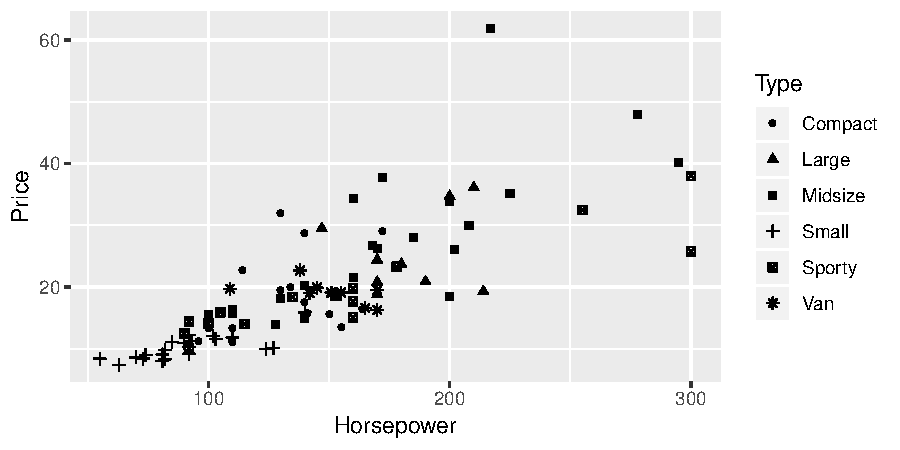
\includegraphics[width=6in]{price_vs_horsepower_by_type}
\end{figure}

\subquestionwithpoints{4} Write ggplot code (as best as you can) to generate this figure.  \spc{5}

Consider the following OLS linear model for target variable \texttt{price}:

\begin{itemize}
\item[\fbox{Model 3}]

\begin{verbatim}
           (Intercept)             Horsepower 
            1.45938866             0.12788635 
             TypeLarge            TypeMidsize 
            5.13487179            -4.98652796 
             TypeSmall             TypeSporty 
            2.42815602             2.23460382 
               TypeVan   Horsepower:TypeLarge 
           25.53605395            -0.02922214 
Horsepower:TypeMidsize   Horsepower:TypeSmall 
            0.04973893            -0.05888501 
 Horsepower:TypeSporty     Horsepower:TypeVan 
           -0.02985597            -0.1807183
\end{verbatim}
\end{itemize}
\subquestionwithpoints{2} What is the \texttt{R} code used to fit Model 3?\spc{1}

\subquestionwithpoints{1} Which model \emph{most likely} has higher $R^2$?

\begin{enumerate}[i)]
\item Model 2
\item Model 3
\item They have equal $R^2$
\item Not enough information to tell
\end{enumerate}

\subquestionwithpoints{2} Which model \emph{most likely} has higher oos$R^2$?

\begin{enumerate}[i)]
\item Model 2
\item Model 3
\item They have equal oos$R^2$
\item Not enough information to tell
\end{enumerate}

\subquestionwithpoints{3} Interpret the number -0.1807183 for term \texttt{Horsepower:TypeVan} in Model 3.\spc{3}

\eenum

\problem This question is about OLS again. For the questions concerned with out of sample, consider running the code using split-sample or gathering future data under stationarity. Consider the following code:

\lstset{basicstyle=\normalsize}
\begin{lstlisting}
n = 100
x = runif(n, 0, 1)
X = cbind(1, x)
beta = c(1, 1)
delta = rnorm(n, mean = 0, sd = 0.1)
y = X % * % beta + delta

mod1 = lm(y ~ 0 + X)
\end{lstlisting}

\benum

\subquestionwithpoints{2} What is $f(x)$ in this case? $f$ is defined as we did in class.\spc{2}

\subquestionwithpoints{3} Circle all the following that are true for \texttt{mod1}.

\begin{enumerate}[i)]
\item $\b$ will be very close to $\beta$
\item $\b$ will not be very close to $\beta$
\item $s_e$ will be very small
\item $s_e$ will not be very small
\item oos$s_e$ will be very small
\item oos$s_e$ will not be very small
\end{enumerate}

Now consider running the following code after running the first chunk of code:\\

\begin{lstlisting}
x_prime = x + rnorm(n, mean = 0, sd = 1e-6)
X = cbind(X, x_prime)
mod2 = lm(y ~ 0 + X)
\end{lstlisting}

\subquestionwithpoints{1} In the case of model 2, what is $p$?\spc{1}

\subquestionwithpoints{4} Circle all the following that are true for \texttt{mod2}.

\begin{enumerate}[i)]
\item $\b$ will be very close to $\beta$
\item $\b$ will not be very close to $\beta$
\item $s_e$ will be very small
\item $s_e$ will not be very small
\item oos$s_e$ will be very small
\item oos$s_e$ will not be very small
\end{enumerate}

Now consider running the following code after running the two previous chunks of code:\\

\begin{lstlisting}
mod3 = lm(y ~ poly(x, 6))
\end{lstlisting}

\subquestionwithpoints{4} Circle all the following that are true for \texttt{mod3}.

\begin{enumerate}[i)]
\item $\b$ will be very close to $\beta$
\item $\b$ will not be very close to $\beta$
\item $s_e$ will be very small
\item $s_e$ will not be very small
\item oos$s_e$ will be very small
\item oos$s_e$ will not be very small
\end{enumerate}

\eenum

\problem This question is about the concept of model validation and the strategy we discussed in class. Let's say we divide scramble the rows of $\mathbb{D}$ then create a partition 

\beqn
\mathbb{D} = \fivevec{\mathbb{D}_{\text{train}}}{\text{------}}{\mathbb{D}_{\text{select}}}{\text{------}}{\mathbb{D}_{\text{test}}}
\eeqn

\noindent in a 3:1:1 ratio train : select : test (in number of rows). 

We then fit $g_1 = \mathcal{A}(\mathcal{H}, \mathbb{D}_{\text{train}})$, $g_2 = \mathcal{A}(\mathcal{H}, \mathbb{D}_{\text{test}})$ and $g_{\text{final}} = \mathcal{A}(\mathcal{H}, \mathbb{D})$. Which of the following statement(s) can be employed as a means of \textit{honest} model validation?

\benum
\subquestionwithpoints{3} We wish to select a model out of $M$ candidate models $g_1, g_2, \ldots, g_M$. Which of the following are recommended strategies of doing so?

\begin{enumerate}[i)]
\item Fitting $g_1, g_2, \ldots, g_M$ to $\mathbb{D}_{\text{train}}$ and then testing on $\mathbb{D}_{\text{train}}$ and then choosing the model with lowest error on $\mathbb{D}_{\text{train}}$.
\item Fitting $g_1, g_2, \ldots, g_M$ to $\mathbb{D}_{\text{train}}$ and then testing on $\mathbb{D}$ and then choosing the model with lowest error on $\mathbb{D}$.
\item Fitting $g_1, g_2, \ldots, g_M$ to $\mathbb{D}_{\text{train}}$ and then testing on $\mathbb{D}_{\text{select}}$ and then choosing the model with lowest error on $\mathbb{D}_{\text{select}}$.
\item Fitting $g_1, g_2, \ldots, g_M$ to $\mathbb{D}_{\text{train}}$ and then testing on $\mathbb{D}_{\text{select}}$ and then $\mathbb{D}_{\text{test}}$ and then choosing the model with lowest error on $\mathbb{D}_{\text{test}}$.
\end{enumerate}

\subquestionwithpoints{3} We wish to select a model out of $M$ candidate models $g_1, g_2, \ldots, g_M$ and then provide an estimate of model generalization error. Which of the following are recommended strategies of doing so?

\begin{enumerate}[i)]
\item Fitting $g_1, g_2, \ldots, g_M$ to $\mathbb{D}_{\text{train}}$ and then testing on $\mathbb{D}_{\text{select}}$ and then choosing the model with lowest error on $\mathbb{D}_{\text{select}}$ and providing the estimate of that error.
\item Fitting $g_1, g_2, \ldots, g_M$ to $\mathbb{D}_{\text{train}}$ and then testing on $\mathbb{D}_{\text{select}}$ and then choosing the model with lowest error on $\mathbb{D}_{\text{select}}$ and then testing on $\mathbb{D}$ and providing the estimate using that error.
\item Fitting $g_1, g_2, \ldots, g_M$ to $\mathbb{D}_{\text{train}}$ and then testing on $\mathbb{D}_{\text{select}}$ and then choosing the model with lowest error on $\mathbb{D}_{\text{select}}$ and then testing on $\mathbb{D}_{\text{test}}$ and providing the estimate using that error.
\item Fitting $g_1, g_2, \ldots, g_M$ to $\mathbb{D}_{\text{train}}$ and then testing on $\mathbb{D}_{\text{select}}$ and then $\mathbb{D}_{\text{test}}$ and then choosing the model with lowest error on $\mathbb{D}_{\text{test}}$ and providing the estimate using that error.
\end{enumerate}

\subquestionwithpoints{2} Would your answer in (b) be able to provide an estimate of the variability in the generalization error? Yes / No.\spc{-0.5}

Consider the selection of the model $g_1, g_2, \ldots, g_M$ to be termed \qu{tuning}. Imagine we used the protocol pictured below.

\begin{figure}[htp]
\centering
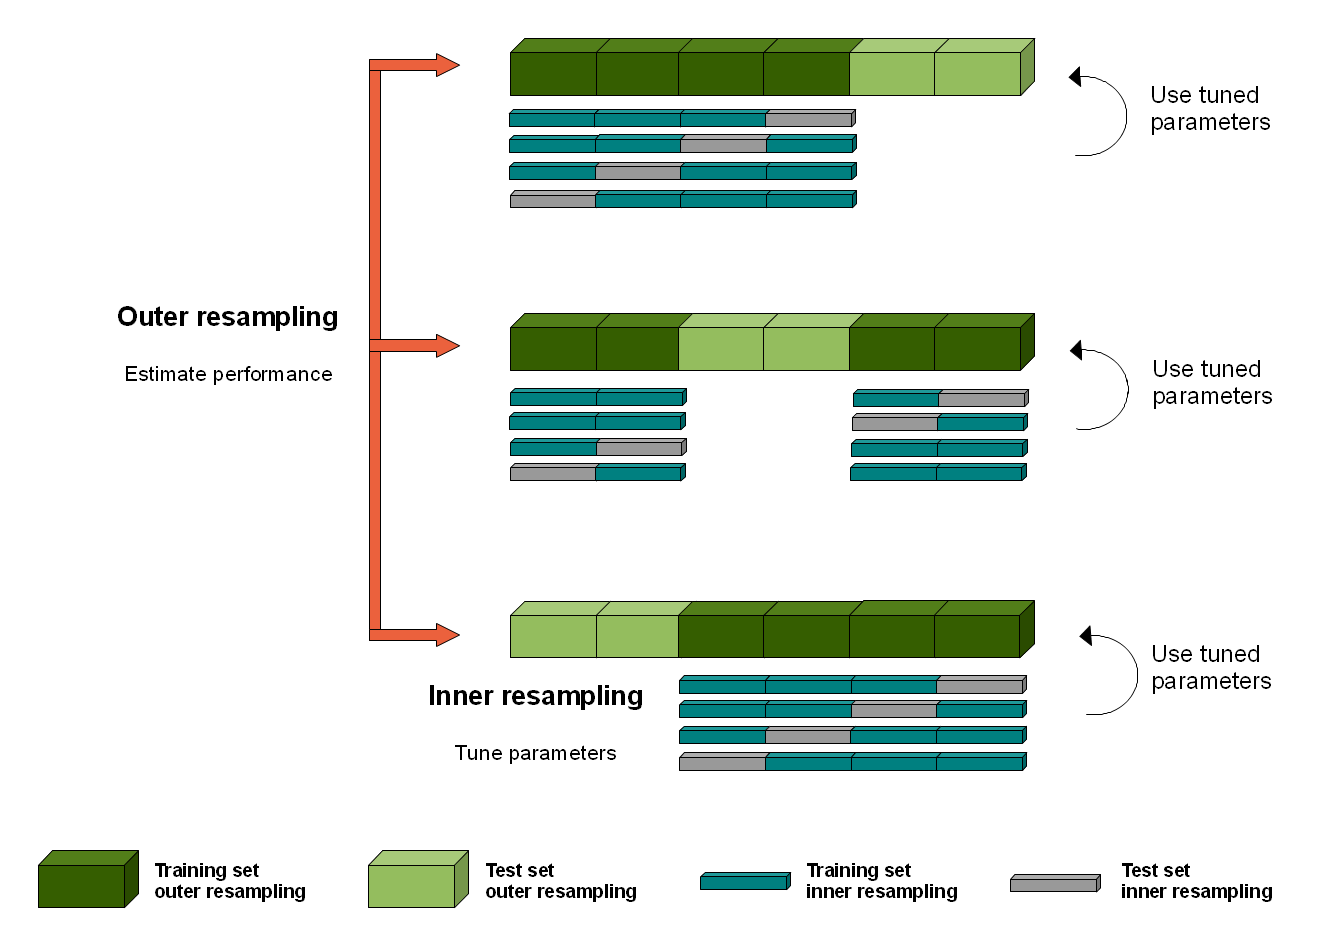
\includegraphics[width=6in]{nested_resampling.png}
\end{figure}

\subquestionwithpoints{3} What are the number of folds in the inner loop and the outer loop \textit{in our problem} respecting the ratio given in the problem description?\spc{3}

\subquestionwithpoints{4} What are the two main advantages of the protocol above over the answer you gave in (b)?\spc{3}




\eenum

\problem Consider the following code:

\begin{lstlisting}
compute_distance_matrix = function(X){
  n = nrow(X)
  D = matrix(NA, n, n)
  for (i_1 in 1 : (n - 1)){
    for (i_2 in (i_1 + 1) : n){
      D[i_1, i_2] = sqrt(sum((X[i_1, ] - X[i_2, ])^2))
    }
  }
  D
}

pacman::p_load(Rcpp)
cppFunction('
  NumericMatrix compute_distance_matrix_cpp(NumericMatrix X) {
    int n = X.nrow();
    int p = X.ncol();
    NumericMatrix D(n, n);
    std::fill(D.begin(), D.end(), NA_REAL);

    for (int i_1 = 0; i_1 < (n - 1); i_1++){
      for (int i_2 = i_1 + 1; i_2 < n; i_2++){
        int sqd_diff = 0;
        for (int j = 0; j < p; j++){
          sqd_diff += pow(X(i_1, j) - X(i_2, j), 2);
        }
        D(i_1, i_2) = sqrt(sqd_diff); 
      }
    }
    return D;
  }
')
\end{lstlisting}

\noindent We now profile both functions using a matrix $\X$ that has $n$ in the 100's via the code: \\

\begin{lstlisting}
system.time({
  D = compute_distance_matrix(X)
})
system.time({
  D = compute_distance_matrix_cpp(X)
})
\end{lstlisting}

\benum

\subquestionwithpoints{2} Which function registers a faster profiling time and by how much? Provide a multiple.\spc{1}

\subquestionwithpoints{2} Explain why this should be.\spc{3}

\subquestionwithpoints{2} You wish to recode the \texttt{R} function \texttt{sort} using \texttt{Rcpp}. Assume your C++ code is bug-free. Is this endeavor fruitful? Why or why not?\spc{3}
\eenum

\problem Consider the following dataset:

\lstset{basicstyle=\footnotesize}
\begin{lstlisting}
> pacman::p_load(ggplot2, dplyr, magrittr)
> D = ggplot2::txhousing
> dim(D)
[1] 8602    9
> summary(D)
    city                year          month       
 Length:8602        Min.   :2000   Min.   : 1.000  
 Class :character   1st Qu.:2003   1st Qu.: 3.000  
 Mode  :character   Median :2007   Median : 6.000  
                    Mean   :2007   Mean   : 6.406  
                    3rd Qu.:2011   3rd Qu.: 9.000  
                    Max.   :2015   Max.   :12.000  
                                                   
     sales            volume              median      
 Min.   :   6.0   Min.   :8.350e+05   Min.   : 50000  
 1st Qu.:  86.0   1st Qu.:1.084e+07   1st Qu.:100000  
 Median : 169.0   Median :2.299e+07   Median :123800  
 Mean   : 549.6   Mean   :1.069e+08   Mean   :128131  
 3rd Qu.: 467.0   3rd Qu.:7.512e+07   3rd Qu.:150000  
 Max.   :8945.0   Max.   :2.568e+09   Max.   :304200  
 NAs   :568     NAs   :568       NAs   :616     
    listings       inventory           date     
 Min.   :    0   Min.   : 0.000   Min.   :2000  
 1st Qu.:  682   1st Qu.: 4.900   1st Qu.:2004  
 Median : 1283   Median : 6.200   Median :2008  
 Mean   : 3217   Mean   : 7.175   Mean   :2008  
 3rd Qu.: 2954   3rd Qu.: 8.150   3rd Qu.:2012  
 Max.   :43107   Max.   :55.900   Max.   :2016  
 NAs   :1424     NAs   :1467                   
\end{lstlisting}
\vspace{-1cm}

\benum

\subquestionwithpoints{2} Write \texttt{dplyr} code below to update \texttt{D} to convert the city variable into a nominal factor variable. \spc{2}

\subquestionwithpoints{5} Write \texttt{dplyr} code below to update \texttt{D} to create a new character variable called \texttt{month\_date} which has a string timestamp with format MM/YYYY, then sort by date (earliest first) and then drop columns \texttt{month}, \texttt{year} and \texttt{date}. \spc{4}

\subquestionwithpoints{2} Write \texttt{dplyr} code below to \qu{windsorize} \texttt{D} on the \texttt{volume} variable. This means it will only contain rows that are between the 5\%ile and 95\%ile of volumes. \spc{2}

\subquestionwithpoints{3} Write \texttt{dplyr} code below to summarize the data in \texttt{D} by providing the average volume in each month. \spc{2}

We now wish to predict the target \texttt{volume} based on the other variables as features. Consider the following code after the first chunk has been executed:

\begin{lstlisting}
> D % <> % na.omit
> pacman::p_load(mlr)  
> modeling_task = makeRegrTask(data = D, target = "volume")
> algorithm = makeLearner("regr.lm")
> validation = makeResampleDesc("CV", iters = 5)
> resample(algorithm, modeling_task, validation, measures = list(rmse))$aggr
34120325
\end{lstlisting}

\subquestionwithpoints{3} Interpret the output, 34120325, as best as you can. \spc{2}

\subquestionwithpoints{2} What simple transformation can be done to one of the variables in the dataset that would likely increase predictive performance?\spc{2}

Consider the following code:

\begin{lstlisting}
> X = model.matrix(volume ~ . * . * ., D)
\end{lstlisting}


\subquestionwithpoints{2} In one sentence (or less) answer the following: which procedure could you use to build a model predicting \texttt{volume} based on the features now found in the design matrix \texttt{X}?\spc{2}
\eenum

\end{document}
